
%% bare_conf.tex
%% V1.4b
%% 2015/08/26
%% by Michael Shell
%% See:
%% http://www.michaelshell.org/
%% for current contact information.
%%
%% This is a skeleton file demonstrating the use of IEEEtran.cls
%% (requires IEEEtran.cls version 1.8b or later) with an IEEE
%% conference paper.
%%
%% Support sites:
%% http://www.michaelshell.org/tex/ieeetran/
%% http://www.ctan.org/pkg/ieeetran
%% and
%% http://www.ieee.org/

%%*************************************************************************
%% Legal Notice:
%% This code is offered as-is without any warranty either expressed or
%% implied; without even the implied warranty of MERCHANTABILITY or
%% FITNESS FOR A PARTICULAR PURPOSE! 
%% User assumes all risk.
%% In no event shall the IEEE or any contributor to this code be liable for
%% any damages or losses, including, but not limited to, incidental,
%% consequential, or any other damages, resulting from the use or misuse
%% of any information contained here.
%%
%% All comments are the opinions of their respective authors and are not
%% necessarily endorsed by the IEEE.
%%
%% This work is distributed under the LaTeX Project Public License (LPPL)
%% ( http://www.latex-project.org/ ) version 1.3, and may be freely used,
%% distributed and modified. A copy of the LPPL, version 1.3, is included
%% in the base LaTeX documentation of all distributions of LaTeX released
%% 2003/12/01 or later.
%% Retain all contribution notices and credits.
%% ** Modified files should be clearly indicated as such, including  **
%% ** renaming them and changing author support contact information. **
%%*************************************************************************


% *** Authors should verify (and, if needed, correct) their LaTeX system  ***
% *** with the testflow diagnostic prior to trusting their LaTeX platform ***
% *** with production work. The IEEE's font choices and paper sizes can   ***
% *** trigger bugs that do not appear when using other class files.       ***                          ***
% The testflow support page is at:
% http://www.michaelshell.org/tex/testflow/



\documentclass[conference, compsoc]{IEEEtran}
% Some Computer Society conferences also require the compsoc mode option,
% but others use the standard conference format.
%
% If IEEEtran.cls has not been installed into the LaTeX system files,
% manually specify the path to it like:
% \documentclass[conference]{../sty/IEEEtran}

% Some very useful LaTeX packages include:
% (uncomment the ones you want to load)


% *** MISC UTILITY PACKAGES ***
%
%\usepackage{ifpdf}
% Heiko Oberdiek's ifpdf.sty is very useful if you need conditional
% compilation based on whether the output is pdf or dvi.
% usage:
% \ifpdf
%   % pdf code
% \else
%   % dvi code
% \fi
% The latest version of ifpdf.sty can be obtained from:
% http://www.ctan.org/pkg/ifpdf
% Also, note that IEEEtran.cls V1.7 and later provides a builtin
% \ifCLASSINFOpdf conditional that works the same way.
% When switching from latex to pdflatex and vice-versa, the compiler may
% have to be run twice to clear warning/error messages.


% *** CITATION PACKAGES ***
%
%\usepackage{cite}
\usepackage{cite}
%\bibliographystyle{ieeetr}
%\usepackage[sorting=none]{biblatex}
%\bibliography{journals,phd-references}
% cite.sty was written by Donald Arseneau
% V1.6 and later of IEEEtran pre-defines the format of the cite.sty package
% \cite{} output to follow that of the IEEE. Loading the cite package will
% result in citation numbers being automatically sorted and properly
% "compressed/ranged". e.g., [1], [9], [2], [7], [5], [6] without using
% cite.sty will become [1], [2], [5]--[7], [9] using cite.sty. cite.sty's
% \cite will automatically add leading space, if needed. Use cite.sty's
% noadjust option (cite.sty V3.8 and later) if you want to turn this off
% such as if a citation ever needs to be enclosed in parenthesis.
% cite.sty is already installed on most LaTeX systems. Be sure and use
% version 5.0 (2009-03-20) and later if using hyperref.sty.
% The latest version can be obtained at:
% http://www.ctan.org/pkg/cite
% The documentation is contained in the cite.sty file itself.






% *** GRAPHICS RELATED PACKAGES ***
%
\ifCLASSINFOpdf
  %\usepackage[pdftex]{graphicx}
  % declare the path(s) where your graphic files are
  %\graphicspath{{pdf/}{jpeg/}}
  % and their extensions so you won't have to specify these with
  % every instance of \includegraphics
  % \DeclareGraphicsExtensions{.pdf,.jpeg,.png}
  %\DeclareGraphicsExtensions{.pdf,.jpeg,.png}
\else
  % or other class option (dvipsone, dvipdf, if not using dvips). graphicx
  % will default to the driver specified in the system graphics.cfg if no
  % driver is specified.
  % \usepackage[dvips]{graphicx}
  % declare the path(s) where your graphic files are
  % \graphicspath{{../eps/}}
  % and their extensions so you won't have to specify these with
  % every instance of \includegraphics
  % \DeclareGraphicsExtensions{.eps}
  %\usepackage{subfigure}
\fi
\usepackage{balance}
\usepackage{graphicx}
\usepackage{multirow}
\usepackage{booktabs}

% graphicx was written by David Carlisle and Sebastian Rahtz. It is
% required if you want graphics, photos, etc. graphicx.sty is already
% installed on most LaTeX systems. The latest version and documentation
% can be obtained at: 
% http://www.ctan.org/pkg/graphicx
% Another good source of documentation is "Using Imported Graphics in
% LaTeX2e" by Keith Reckdahl which can be found at:
% http://www.ctan.org/pkg/epslatex
%
% latex, and pdflatex in dvi mode, support graphics in encapsulated
% postscript (.eps) format. pdflatex in pdf mode supports graphics
% in .pdf, .jpeg, .png and .mps (metapost) formats. Users should ensure
% that all non-photo figures use a vector format (.eps, .pdf, .mps) and
% not a bitmapped formats (.jpeg, .png). The IEEE frowns on bitmapped formats
% which can result in "jaggedy"/blurry rendering of lines and letters as
% well as large increases in file sizes.
%
% You can find documentation about the pdfTeX application at:
% http://www.tug.org/applications/pdftex





% *** MATH PACKAGES ***
%
\usepackage{amsmath}
\DeclareMathOperator*{\argmin}{arg\,min} % thin space, limits underneath in displays
\DeclareMathOperator*{\argmax}{arg\,max} % thin space, limits underneath in displays
\newcommand{\ineq}{%
	\mathrel{\mkern1mu\underline{\mkern-1mu\in\mkern-1mu}\mkern1mu}}
%\DeclareMathOperator*{\argmin}{argmin} % no space, limits underneath in displays
%\DeclareMathOperator{\argmin}{arg\,min} % thin space, limits on side in displays
%\DeclareMathOperator{\argmin}{argmin} % no space, limits on side in displays
% A popular package from the American Mathematical Society that provides
% many useful and powerful commands for dealing with mathematics.
%
% Note that the amsmath package sets \interdisplaylinepenalty to 10000
% thus preventing page breaks from occurring within multiline equations. Use:
%\interdisplaylinepenalty=2500
% after loading amsmath to restore such page breaks as IEEEtran.cls normally
% does. amsmath.sty is already installed on most LaTeX systems. The latest
% version and documentation can be obtained at:
% http://www.ctan.org/pkg/amsmath





% *** SPECIALIZED LIST PACKAGES ***
%
\usepackage{algorithmic}
% algorithmic.sty was written by Peter Williams and Rogerio Brito.
% This package provides an algorithmic environment fo describing algorithms.
% You can use the algorithmic environment in-text or within a figure
% environment to provide for a floating algorithm. Do NOT use the algorithm
% floating environment provided by algorithm.sty (by the same authors) or
% algorithm2e.sty (by Christophe Fiorio) as the IEEE does not use dedicated
% algorithm float types and packages that provide these will not provide
% correct IEEE style captions. The latest version and documentation of
% algorithmic.sty can be obtained at:
% http://www.ctan.org/pkg/algorithms
% Also of interest may be the (relatively newer and more customizable)
% algorithmicx.sty package by Szasz Janos:
% http://www.ctan.org/pkg/algorithmicx




% *** ALIGNMENT PACKAGES ***
%
\usepackage{array}
% Frank Mittelbach's and David Carlisle's array.sty patches and improves
% the standard LaTeX2e array and tabular environments to provide better
% appearance and additional user controls. As the default LaTeX2e table
% generation code is lacking to the point of almost being broken with
% respect to the quality of the end results, all users are strongly
% advised to use an enhanced (at the very least that provided by array.sty)
% set of table tools. array.sty is already installed on most systems. The
% latest version and documentation can be obtained at:
% http://www.ctan.org/pkg/array


% IEEEtran contains the IEEEeqnarray family of commands that can be used to
% generate multiline equations as well as matrices, tables, etc., of high
% quality.




% *** SUBFIGURE PACKAGES ***
\ifCLASSOPTIONcompsoc
  \usepackage[caption=false,font=normalsize,labelfont=sf,textfont=sf]{subfig}
\else
  \usepackage[caption=false,font=footnotesize]{subfig}
\fi
% subfig.sty, written by Steven Douglas Cochran, is the modern replacement
% for subfigure.sty, the latter of which is no longer maintained and is
% incompatible with some LaTeX packages including fixltx2e. However,
% subfig.sty requires and automatically loads Axel Sommerfeldt's caption.sty
% which will override IEEEtran.cls' handling of captions and this will result
% in non-IEEE style figure/table captions. To prevent this problem, be sure
% and invoke subfig.sty's "caption=false" package option (available since
% subfig.sty version 1.3, 2005/06/28) as this is will preserve IEEEtran.cls
% handling of captions.
% Note that the Computer Society format requires a larger sans serif font
% than the serif footnote size font used in traditional IEEE formatting
% and thus the need to invoke different subfig.sty package options depending
% on whether compsoc mode has been enabled.
%
% The latest version and documentation of subfig.sty can be obtained at:
% http://www.ctan.org/pkg/subfig




% *** FLOAT PACKAGES ***

%\usepackage{fixltx2e}
% fixltx2e, the successor to the earlier fix2col.sty, was written by
% Frank Mittelbach and David Carlisle. This package corrects a few problems
% in the LaTeX2e kernel, the most notable of which is that in current
% LaTeX2e releases, the ordering of single and double column floats is not
% guaranteed to be preserved. Thus, an unpatched LaTeX2e can allow a
% single column figure to be placed prior to an earlier double column
% figure.
% Be aware that LaTeX2e kernels dated 2015 and later have fixltx2e.sty's
% corrections already built into the system in which case a warning will
% be issued if an attempt is made to load fixltx2e.sty as it is no longer
% needed.
% The latest version and documentation can be found at:
% http://www.ctan.org/pkg/fixltx2e


%\usepackage{stfloats}
% stfloats.sty was written by Sigitas Tolusis. This package gives LaTeX2e
% the ability to do double column floats at the bottom of the page as well
% as the top. (e.g., "\begin{figure*}[!b]" is not normally possible in
% LaTeX2e). It also provides a command:
%\fnbelowfloat
% to enable the placement of footnotes below bottom floats (the standard
% LaTeX2e kernel puts them above bottom floats). This is an invasive package
% which rewrites many portions of the LaTeX2e float routines. It may not work
% with other packages that modify the LaTeX2e float routines. The latest
% version and documentation can be obtained at:
% http://www.ctan.org/pkg/stfloats
% Do not use the stfloats baselinefloat ability as the IEEE does not allow
% \baselineskip to stretch. Authors submitting work to the IEEE should note
% that the IEEE rarely uses double column equations and that authors should try
% to avoid such use. Do not be tempted to use the cuted.sty or midfloat.sty
% packages (also by Sigitas Tolusis) as the IEEE does not format its papers in
% such ways.
% Do not attempt to use stfloats with fixltx2e as they are incompatible.
% Instead, use Morten Hogholm'a dblfloatfix which combines the features
% of both fixltx2e and stfloats:
%
% \usepackage{dblfloatfix}
% The latest version can be found at:
% http://www.ctan.org/pkg/dblfloatfix


\usepackage[english]{babel}
\usepackage{blindtext}

% *** PDF, URL AND HYPERLINK PACKAGES ***
%
\usepackage{url}
% url.sty was written by Donald Arseneau. It provides better support for
% handling and breaking URLs. url.sty is already installed on most LaTeX
% systems. The latest version and documentation can be obtained at:
% http://www.ctan.org/pkg/url
% Basically, \url{my_url_here}.


% *** Do not adjust lengths that control margins, column widths, etc. ***
% *** Do not use packages that alter fonts (such as pslatex).         ***
% There should be no need to do such things with IEEEtran.cls V1.6 and later.
% (Unless specifically asked to do so by the journal or conference you plan
% to submit to, of course. )


% correct bad hyphenation here
\hyphenation{op-tical networks semi-conduc-tor}
\hyphenation{PASCAL}

\begin{document}
%
% paper title
% Titles are generally capitalized except for words such as a, an, and, as,
% at, but, by, for, in, nor, of, on, or, the, to and up, which are usually
% not capitalized unless they are the first or last word of the title.
% Linebreaks \\ can be used within to get better formatting as desired.
% Do not put math or special symbols in the title.
\title{Batik Classification using Deep Convolutional Network Transfer Learning}
% author names and affiliations
% use a multiple column layout for up to three different
% affiliations

\author{\IEEEauthorblockN{Yohanes Gultom, Aniati Murni Arymurthy\\\\}
	\IEEEauthorblockA{
		\normalfont Faculty of Computer Science, Universitas Indonesia\\\\
		\textit{yohanes.gultom@ui.ac.id} \\
		\textit{aniati@cs.ui.ac.id}
	} \\
}

% conference papers do not typically use \thanks and this command
% is locked out in conference mode. If really needed, such as for
% the acknowledgment of grants, issue a \IEEEoverridecommandlockouts
% after \documentclass

% for over three affiliations, or if they all won't fit within the width
% of the page, use this alternative format:
% 
%\author{\IEEEauthorblockN{Michael Shell\IEEEauthorrefmark{1},
%Homer Simpson\IEEEauthorrefmark{2},
%James Kirk\IEEEauthorrefmark{3}, 
%Montgomery Scott\IEEEauthorrefmark{3} and
%Eldon Tyrell\IEEEauthorrefmark{4}}
%\IEEEauthorblockA{\IEEEauthorrefmark{1}School of Electrical and Computer Engineering\\
%Georgia Institute of Technology,
%Atlanta, Georgia 30332--0250\\ Email: see http://www.michaelshell.org/contact.html}
%\IEEEauthorblockA{\IEEEauthorrefmark{2}Twentieth Century Fox, Springfield, USA\\
%Email: homer@thesimpsons.com}
%\IEEEauthorblockA{\IEEEauthorrefmark{3}Starfleet Academy, San Francisco, California 96678-2391\\
%Telephone: (800) 555--1212, Fax: (888) 555--1212}
%\IEEEauthorblockA{\IEEEauthorrefmark{4}Tyrell Inc., 123 Replicant Street, Los Angeles, California 90210--4321}}

% use for special paper notices
%\IEEEspecialpapernotice{(Invited Paper)}
% make the title area
%\maketitle
\twocolumn[
{\csname @twocolumnfalse\endcsname \maketitle}
{\csname @twocolumnfalse\endcsname 
	%\input{abstract}
	\renewcommand{\abstractname}{Abstract}
	\begin{abstract}
		\noindent
		\normalfont 
		Batik fabric is one of the most profound cultural heritage in Indonesia. Hence, continuous research on understanding it is necessary to preserve it. Despite of being one of the most common research task, Batik's pattern automatic classification still requires some improvement especially in regards to invariance dilemma. Convolutional neural network (ConvNet) is one of deep learning architecture which able to learn data representation by combining local receptive inputs, weight sharing and convolutions in order to solve invariance dilemma in image classification. Using dataset of 2,092 Batik patches (5 classes), the experiments show that the proposed model, which used deep ConvNet VGG16 as feature extractor (transfer learning), achieves slightly better average of 89$\pm$7\% accuracy than SIFT and SURF-based that achieve 88$\pm$10\% and 88$\pm$8\% respectively. Despite of that, SIFT reaches around 5\% better accuracy in rotated and scaled dataset.
		\\\\
		\noindent
		\textbf{Keywords}: \textit{Batik, classification, deep learning, transfer learning} \\\\
	\end{abstract}
	
	\renewcommand{\abstractname}{Abstrak}
	\begin{abstract}
		\noindent
		\normalfont 
		Kain Batik adalah salah satu warisan kebudayaan Indonesia yang sangat berharga. Oleh karena itu, penelitian yang berkesinambungan perlu dilakukan untuk melestarikannya. Sekalipun telah menjadi topik penelitian yang umum, klasifikasi pola Batik secara otomatis masih memiliki beberapa tantangan yang perlu diselesaikan. Salah satu tantangan tersebut adalah masalah \textit{invariance dilemma}. \textit{Convolutional neural network} (ConvNet) adalah salah satu arsitektur \textit{deep learning} yang mampu mempelajari representasi data dengan mengkombinasikan teknik \textit{local receptive inputs}, \textit{weight sharing} dan \textit{convolutions} untuk mengatasi masalah \textit{invariance dilemma} pada klasifikasi citra seperti pola Batik. Eksperimen menggunakan \textit{dataset} 2,092 potongan foto Batik (5 kelas) menunjukkan bahwa model yang menggunakan ConvNet VGG16 sebagai ekstraktor fitur mencapai rata-rata akurasi 89$\pm$7\% sedangkan model berbasis SIFT dan SURF mencapai rata-rata 88$\pm$10\% dan 88$\pm$8\%. Meskipun demikian, SIFT lebih akurat sekitar 5\% pada \textit{dataset} yang dirotasi dan diperbesar.
		\\\\
		\noindent
		\textbf{Kata Kunci}: \textit{Batik, klasifikasi, deep learning, transfer learning} \\\\
	\end{abstract}
	
	%\begin{IEEEkeywords}
	%%IEEEtran, journal, \LaTeX, paper, template.
	%\end{IEEEkeywords}
}
%\vspace{1cm}
]

% For peer review papers, you can put extra information on the cover
% page as needed:
% \ifCLASSOPTIONpeerreview
% \begin{center} \bfseries EDICS Category: 3-BBND \end{center}
% \fi
%
% For peerreview papers, this IEEEtran command inserts a page break and
% creates the second title. It will be ignored for other modes.
\IEEEpeerreviewmaketitle

\section{Introduction}

Batik fabric is one of the most profound cultural heritage in Indonesia. Hence, continuous research on understanding it is necessary to preserve it. One of the most popular research topic in computer science is batik classification. This topic can not be separated from another crucial subtopic: feature extraction. It is because in order to achieve high classification accuracy, a machine learning model requires numerical features extracted from Batik images.

\begin{figure}[!t]
\centering
\subfloat[Parang]{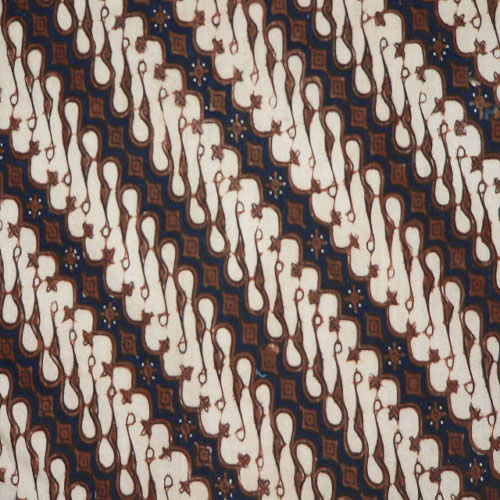
\includegraphics[width=1.0in]{../batik_parang}%
\label{fig_batik_parang}}
\hfil
\subfloat[Kawung]{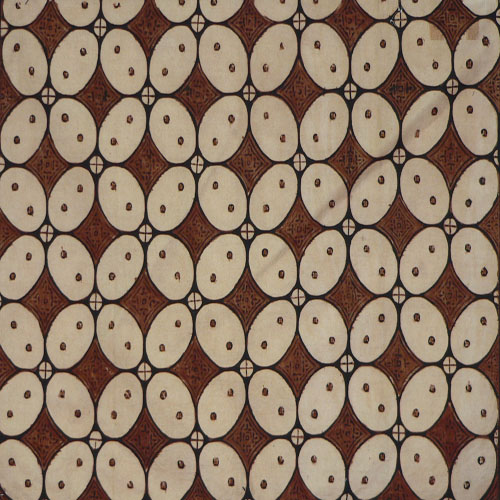
\includegraphics[width=1.0in]{../batik_kawung}%
\label{fig_batik_kawung}}
\hfil
\subfloat[Ceplok]{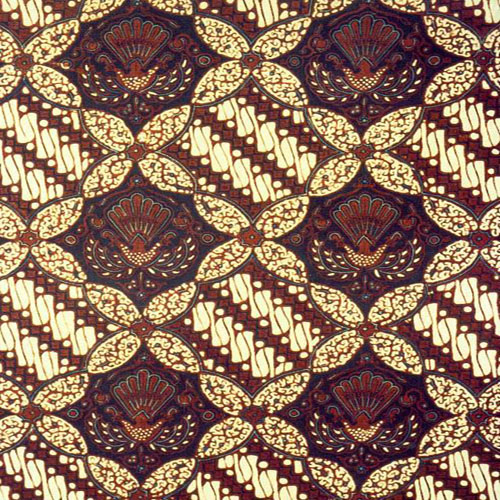
\includegraphics[width=1.0in]{../batik_ceplok}%
\label{fig_batik_ceplok}}
\hfil
\subfloat[Nitik]{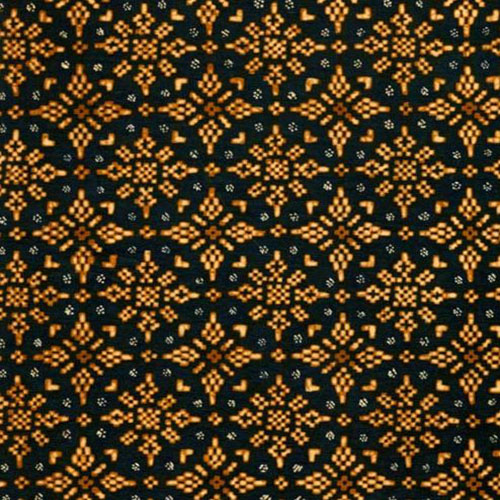
\includegraphics[width=1.0in]{../batik_nitik}%
\label{fig_batik_nitik}}
\hfil
\subfloat[Lereng]{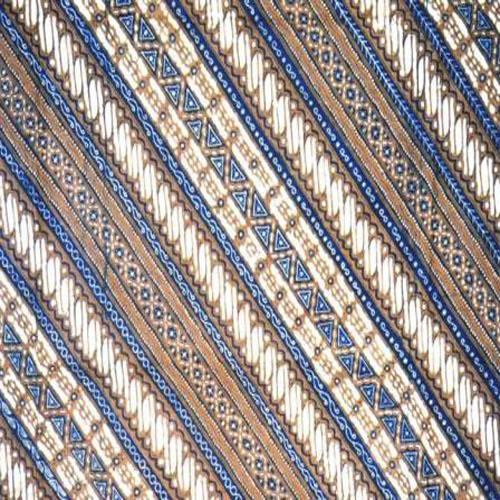
\includegraphics[width=1.0in]{../batik_lereng}%
\label{fig_batik_lereng}}
\caption{General Batik pattern classification}
\label{fig_batik_motifs}
\end{figure}

Since the most prominent feature of Batik is its uniquely recurring pattern (motif), earlier researches have focused on finding a method to extract features from it. Earlier researches have shown good result using several method such as Generalize Hough Transform \cite{sanabila2009recognition}, Gabor, GLCM and LBP \cite{fahmi2016feature}. The recent methods that are currently considered as state of the art are Scale-Invariant Feature Transform (SIFT) \cite{azhar2015batik} \cite{nurhaida2015automatic} and Speeded up robust features (SURF) \cite{willy2013evaluation}. Classifications using other features such as color and contrast are showing potentials but need to be researched further \cite{moertini2005algorithms}.

Deep learning based models have outperformed state-of-the-art methods in many domains including image classification and object recognition \cite{lecun2015deep}. One of the deep learning models, convolutional neural network (convnet) \cite{lecun1998gradient}, is currently considered as the state-of-the-art of image classification model as it was used as the base structure by ILSVRC-2014 top achievers \cite{simonyan2014very}. Therefore convnet has potential to improve result on other image classification problems such as Batik classification.

In this paper, we propose a neural network Batik classification model that uses pre-trained deep convolutional network (VGG16) \cite{simonyan2014very} as a feature extractor. Features from a dataset of five general classes of Indonesian Batik (shown in Figure \ref{fig_batik_motifs}) are extracted using VGG16, SIFT and SURF then classified using several machine learning classifiers. In order to test the capability of the model to solve invariance dilemma, tests are also done with rotated and scaled (zoomed) images.

\section{Related Works}

Recent researches in Batik classification can be divided into two groups: (1) Researches on classification using handcrafted features and (2) researches on classification using automatically extracted features using deep learning.

\subsection{Classification using Handcrafted Features}

Since Batik classification has been researched for quite some time, current available methods are robust enough to noise addition, compression, and retouching of the input images. However most of them are still having difficulties with variance in transformations which involve either translation, rotation, scaling or combinations of them \cite{nurhaida2015automatic}. One of the initial work on Batik Classification was done using Generalized Hough Transform (GHT) to recognize Batik motifs as part of a content-based image retrieval (CBIR) \cite{sanabila2009recognition}. The research focused on detection of repetitive motifs in a batik image but not yet addressed various orientations and scale. 

One of the most recent research address the performance of several feature extraction methods (Gabor filter, log-Gabor filter, Gray Level Co-occurrence Matrix, and Local Binary Pattern) on rotated and scaled primitive Batik motifs \cite{fahmi2016feature}. It shows that applying Principal Component Analysis (PCA) to reduce dimensionality can improve the classification 17\%. It also shows that applying Sequential Forward Floating Selection (SFFS) as feature selection makes the execution time 1,800 times faster.

\begin{figure}[h]
	\begin{center}
		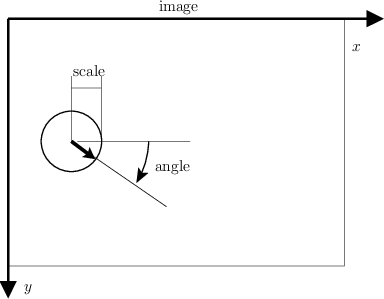
\includegraphics[width=2.0in]{../sift-keypoint}
		\renewcommand{\figurename}{Fig.}		
		\caption{SIFT Keypoint}
		\label{fig_keypoint}
	\end{center}
\end{figure}


Improvements on Batik classification were motivated by the emergence of Scale-Invariant Feature Transform (SIFT)\cite{lowe2004distinctive} and Speeded up robust features (SURF)\cite{bay2006surf}. Both of these keypoint-based feature extraction methods are proposed to solve the transformation invariance dilemma. SIFT keypoint is a circular image region with an orientation which can be obtained by detecting extrema of Difference of Gaussian (DoG) pyramid \cite{lowe2004distinctive}. It's defined by four parameters: center coordinates x and y, scale and its orientation (an angle expressed in radians) as shown in Figure \ref{fig_keypoint}. An image, for example Batik image, may contains multiple keypoints as shown in Figure \ref{fig_keypoint}. In order to be efficiently and effectively used as a feature for classification, the keypoint need to be represented as SIFT descriptor. By definition it is a 3-dimensional spatial histogram of the image gradients characterizing a SIFT keypoint.

\begin{figure}[h]
	\begin{center}
		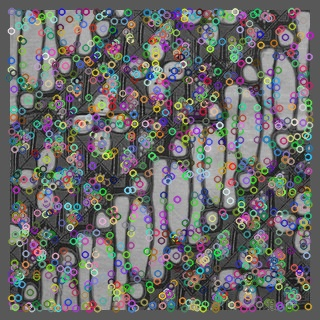
\includegraphics[width=2.0in]{../batik-parang-keypoints}
		\renewcommand{\figurename}{Fig.}		
		\caption{SIFT keypoints in Batik Parang}
		\label{fig_batik_parang_keypoints}
	\end{center}
\end{figure}

Recent research proved that using SIFT descriptors to calculate similarity between Batik images can give 91.53\% accuracy \cite{nurhaida2015automatic}. Voting Hough Transform was also applied to the descriptors to eliminate mismatched keypoint candidates hence improving the accuracy. This research suggested that the original SIFT descriptor matching shouldn't be directly used to calculate similarity of Batik images due to many numbers of mismatched keypoints. This research uses fundamental templates of Batik patterns as a dataset instead of Batik photos. So it does not address issue related to noises which happen on non-processed images such as blur/unfocused, lightning issue, watermarks .etc.

Another research \cite{azhar2015batik} proposed a classification method using support vector machine (SVM) fed by bag of words (BoW) features extracted using SIFT descriptors. In this research, SIFT descriptors also weren't used directly as features for SVM but were clustered using k-means vector quantization algorithm to build vocabularies. These visual vocabularies then used to describe each images and fed to SVM classifier. This approach is required because SIFT descriptors have high dimensionality and vary between each images. The experiment results showed high average accuracy of 97.67\% for normal images, 95.47\% for rotated images and 79\% for scaled images. Besides that SIFT and bag of words made a good feature extractor, this research also concluded that further works need to handle scaled Batik image cases. 

An earlier research \cite{willy2013evaluation} proved that SURF can extract transformation invariant features faster than SIFT for classification of Songket, another Indonesian traditional fabric with motifs just like Batik. Unlike the others, this research used SIFT and SURF features directly to compute the matching scores between Songket images. The scores are calculated by (1) the number of matched keypoints and (2) the average total distance of the n-nearest keypoints. The result of experiments showed that the matching accuracy with SIFT features was 92-100\% and 65-97\% with SURF. With SURF features, the accuracy dropped quite significant if salt and pepper noises were added while SIFT was more stable. Apparently, this one wasn't paying much attention to transformation variance as it didn't apply transformation noise as in other research\cite{azhar2015batik}.


\subsection{Classification using Deep Learning}

Deep learning is a multilayer representation learning in artificial neural network \cite{lecun2015deep}. While representation learning itself is a method in machine learning to automatically extract/learn representation (features) from raw data. The representation of the raw data then can be used for recognition or classification task. Some fundamental deep learning architectures for instances are convolutional neural network (ConvNet), deep belief network (DBN), autoencoder (AE) and recurrent neural network (RNN). Despite of being an old idea, it was recently emerged due to the several factors: (1) discovery of new techniques (eg. pretraining \& dropout) and new activation functions (eg. ReLU), (2) enormous supply of data (big data), and (3) rapid improvement in computational hardware, especially GPU.

Although not yet many, the advent of deep learning also motivated a research on Batik classification using convolutional stacked autoencoder \cite{menzata2014sistem}. This research proposed the usage of convolutional transformations to reduce the input nodes of stacked autoencoder. The experiment showed that this deep architecture was able to achieve 81,73\% accuracy by using small patches of Batik for training. When noises were added its accuracy dropped to 49\% for gaussian noises, 61\% for rotations, 70\% for scalings and 75\% for illumination noises. Another research have shown that deep architecture such as convolutional neural network should be able to outperform handcrafted features such as SIFT\cite{fischer2014descriptor}. Therefore further research on Batik classification using deep learning architectures is encouraged.

\section{Methodology}

We propose a deep convolutional neural network composed by a pre-trained VGG16 (without its top layer) as automatic feature extractor and a multi-layer perceptron (MLP) as classifier. The method of using pre-trained deep network as part of another neural network to solve different (but related) task can be considered as transfer learning or self-taught learning \cite{raina2007self}.

\subsection{Convolutional Neural Network}

Convolutional network is a special kind of neural network optimized to learn representation of an image \cite{lecun2015deep}. It introduces 2 new types of hidden layers: convolutional and subsampling/pooling layers. Each layer in convnet connects neurons (pixels) from their input layer in form of local receptives (square patches) through a shared weights to a feature map \cite{lecun1998gradient}. On top of a set of convolutional and pooling layers, some fully-connected layers are added as classifier as described by Figure \ref{fig_lenet5_convnet}.

\begin{figure}[h]
	\begin{center}
		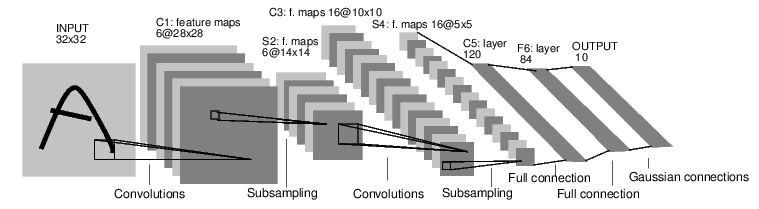
\includegraphics[width=3.0in]{../lenet5}
		\renewcommand{\figurename}{Fig.}		
		\caption{LeNet5 convolutional network}
		\label{fig_lenet5_convnet}
	\end{center}
\end{figure}


VGG16 is a very deep convnet model made by Visual Geometry Group (VGG), University of Oxford \cite{simonyan2014very}. It was trained on 1,000,000 images dataset from ImageNet and achieve state-of-the-art results on Large-Scale Visual Recognition Challenge (ILSVRC) 2014. It contains 16 hidden layers composed of convolutional layers, max pooling layers and fully-connected layers as shown in Figure \ref{fig_vgg16}. The convolution and fully-connected layers uses ReLu activation function (Equation \ref{eq_relu}), except the output layer that uses a SoftMax activation function (Equation \ref{eq_softmax}) to estimate probability of multiple classes/labels. Dropout is also used as regularization after each tanh fully-connected layers to avoid overfitting by randomly drop/turn off (set value to zero) hidden nodes (Equation \ref{eq_dropout}) \cite{srivastava2014dropout}.

\begin{equation}
y_{i}=\log(1+\exp x _{i})
\label{eq_relu}
\end{equation}

\begin{equation}
y_{i}={\frac {e^{x _{i}}}{\sum _{k=1}^K e^{x _{k}}}} \quad \text{, for i=1..K}
\label{eq_softmax}
\end{equation}

\begin{align}
r_{j}^{x} \sim Bernoulli(p), \nonumber \\
\tilde{y} _{i}= r _{i} * y _{i}
\label{eq_dropout}
\end{align}


\begin{figure}[h]
	\begin{center}
		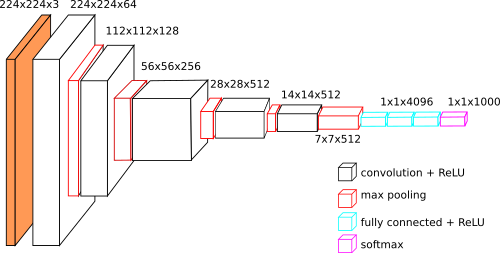
\includegraphics[width=3.0in]{../vgg16}
		\renewcommand{\figurename}{Fig.}		
		\caption{VGG16 deep convolutional network model of Visual Geometry Group, Oxford}
		\label{fig_vgg16}
	\end{center}
\end{figure}

\subsection{Transfer Learning}

Deep neural networks usually requires a lot of training data in order to learn the representation of the data. In case there is not enough training data, there are several techniques to help neural networks model learns data representation using small training data. One of the technique is transferring knowledge of other pre-trained neural network model to our model. This technique is known as transfer learning or self-taught learning \cite{raina2007self}.

Our proposed model uses transferred knowledge (layer weights) from pre-trained VGG16 model (provided by deep learning framework Keras\footnote{\url{https://keras.io/applications/#vgg16}}) which was pre-trained using 1,000,000 images dataset from ImageNet. Intermediate outputs of VGG16 can be used to extract generic features for any image classifier \cite{fischer2014descriptor}. Therefore, even though VGG16 was not designed to classify Batik patterns, it should be able to extract useful generic features from Batik images which can be used further for classification. 

Compared to SIFT/SURF BoW, using pre-trained VGG16 allows us to reduce time needed to extract features because no training required for the feature extractor. Moreover, since our proposed model is based on neural network, execution time may also be reduced significantly by utilizing GPU parallelization.

To improve comprehension and reproducibility, the proposed model and experiment codes are also available in public online code repository\footnote{\url{https://github.com/yohanesgultom/deep-learning-batik-classification}}. This research also utilizes opensource TensorFlow-backed Keras as deep learning framework and scikit-learn\footnote{\url{http://scikit-learn.org/}} library for classification and evaluation to reduce amount of codes written so they can be easily studied further.

\section{Experiments and Results}

In order to measure the performance of our model, we trained our model and compared it with SIFT and SURF based models.

\subsection{Experiments}

The dataset used in the experiments originally comes from Machine Learning and Computer Vision (MLCV) Lab, Faculty of Computer Science, University of Indonesia. The original dataset consists of 603 Batik photos ($\pm$ 78.3 MB) gathered from various sources thus having different size, quality and view angle. But based on the previous research, this dataset is expanded by equally slicing each images to four patches (Figure \ref{fig_dateset}) for better accuracy \cite{menzata2014sistem}. Hence, the dataset used in the experiments contains 2,092 images (patches) of five classes:

\begin{enumerate}
\item Ceplok: 504 images
\item Kawung: 368 images
\item Lereng: 220 images
\item Nitik: 428 images
\item Parang: 572 images
\end{enumerate}


\begin{figure}[h]
	\begin{center}
		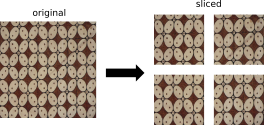
\includegraphics[width=3.0in]{../dataset}
		\renewcommand{\figurename}{Fig.}
		\caption{Example of generation of Batik patches}
		\label{fig_dateset}
	\end{center}
\end{figure}


In the first experiment, the objectives are to compare our performance of SIFT, SURF and VGG16 extractors on the dataset by using the result to train and test six different classifiers: Logistic Regression, Support Vector Machine (RBF Kernel), Multi-Layer Perceptron (1 ReLU hidden layer, 100 nodes), Decision Tree, Gradient Boosting and Random Forest. The dataset is minimally preprocessed by converting each images to grayscale before processed by three extractors:

\begin{enumerate}
\item SIFT Bag of Words (BoW): extracts 2,800 features
\item SURF Bag of Words (BoW): extracts 2,800 features
\item VGG16: extracts 512 features
\end{enumerate}

%Our neural network classifier was trained for 50 epoch using Cross Entropy function to calculate loss (Equation \ref{eq_cross_entropy_loss}) and optimized using Stochastic Gradient Descent (SGD) (Equation \ref{eq_sgd}) to update weights.
%
%\begin{equation}
%V(f(\vec{x}),t) = -t\ln(f(\vec{x}))-(1-t)\ln(1-f(\vec{x}))
%\label{eq_cross_entropy_loss}
%\end{equation}
%
%\begin{equation}
%w:=w-\eta \nabla Q_{i}(w)+\alpha \Delta w
%\label{eq_sgd}
%\end{equation}

\begin{figure}[h]
	\begin{center}
		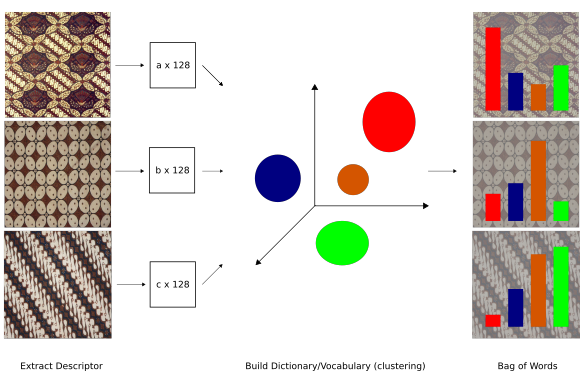
\includegraphics[width=3.0in]{../sift-bag-of-words}
		\renewcommand{\figurename}{Fig.}	
		\caption{SIFT for building bag of words visual vocabularies}
		\label{fig_sift_bag_of_words}
	\end{center}
\end{figure}

While, VGG16 extractor does not require any training because pre-trained model (weights) are used, the SIFT and SURF features extractors are trained using the best methods (achieving highest accuracy) described in previous research \cite{azhar2015batik} (illustrated in Figure \ref{fig_sift_bag_of_words}):

\begin{enumerate}
	\item Image descriptors were extracted according to their feature extractor (SIFT or SURF)
	\item Descriptors were clustered to 2,800 clusters using K-Means to get visual vocabularies for Bag of Words (BoW)
	\item Those 2,800 visual vocabularies then used to compute BoW features from SIFT/SURF image descriptors to produce 2,800 features
\end{enumerate} 

In the first experiment, each extracted features are used to train and test six different classifiers mentioned above using 10 folds cross validation. So effectively, each classifiers are trained using 1,883 images and tested using 209 images 10 times. The results are averaged and then compared to see which combination of extractor and classifier performs the best.

The best combinations of each three extractors from first experiment are tested for their capability to handle invariance dillema in the second experiment. The steps of experiments are below:

\begin{enumerate}
	\item Each combinations of the best extractors-classifiers are trained using 2,092 images (without any transformation)
	\item A subset of 193 images are randomly chosen from dataset and transformed to six test dataset by applying six transformations: 
	\begin{enumerate}
		\item 90$^{\circ}$ rotation
		\item 180$^{\circ}$ rotation
		\item 270$^{\circ}$ rotation
		\item 10\% zoom-in (1.1 scale)
		\item 30\% zoom-in (1.3 scale)
		\item 50\% zoom-in (1.5 scale)										
	\end{enumerate}
	\item Each combinations of the best extractors-classifiers are tested against those six transformed test dataset
\end{enumerate}

All experiments were conducted using Intel Core i7-5960X CPU, 66 GB RAM, NVIDIA GTX 980 4GB GPU, 240GB SSD, Debian 8 OS. The VGG16 extractor runs on GPU to reduce the execution time but the result should not be different than running it on CPU. 

\subsection{Results and Analysis}

In the first experiment, the proposed model (VGG16 MLP), achieved slightly better (1\%) accuracy and less deviation than the best SIFT and SURF models (SIFT LogReg and SURF MLP) as shown by chart in Figure \ref{fig_accuracy_comparison}. The average accuracy achieved by the proposed model is also $\pm$8\% better than Stacked-Autoencoder \cite{menzata2014sistem} that used dataset from same origin.

On general, the result also shows that VGG16 extractor performs as well as SIFT and SURF extractors despite of fewer features dimension (512 features against 2,800 features). Since VGG16 extractor doesn't require training, it is more efficient than SIFT/SURF BoW extractor. On top of that, neural network models such as VGG16 are known to run parallelly in GPU \cite{krizhevsky2012imagenet} to make it event more efficient. 

It is also shown that decision-tree-based classifiers (Decision Tree, Random Forest and Gradient Boosting) generally achieve lower accuracy compared to non-decision-tree classifiers. Only SIFT Gradient Boosting and VGG Gradient Boosting which outperform SVM classifiers. This shows that the extracted features don't have nominal scale which is usually suitable with decision-tree-based classifiers. Meanwhile, SVM, which represents non-linear classifier, is outperformed by logistic regression and single layer ReLU MLP that represent linear classifier. This result shows that the features extracted by SIFT, SURF and VGG16 are not linearly separable.

In the second experiment, the proposed model (VGG16 MLP) shows slightly less accurate results compared to SIFT and SURF models. For rotated and zoomed-in datasets, SIFT model is $\pm$5\% better than VGG16 model. While SURF model is $\pm$5\% better than VGG16 only on rotated datasets but $\pm$3\% worse than it. Despite of that, the accuracies of the proposed model are generally high (above 80\%) and much better than self-trained Stacked-Autoencoder from previous research \cite{menzata2014sistem}. This shows that pre-trained VGG16 is able to handle invariance dilemma in Batik images almost as good as SIFT and SURF extractor.

\begin{figure}[t]
	\begin{center}
		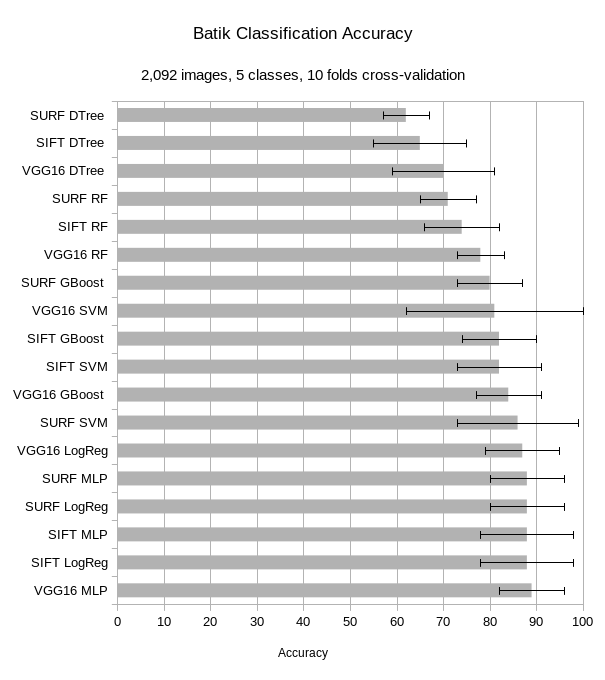
\includegraphics[width=3.5in]{../chart_accuracy_rev}
		\renewcommand{\figurename}{Fig.}
		\caption{Models accuracy comparison}
		\label{fig_accuracy_comparison}
	\end{center}
\end{figure}

\begin{table}[t]
	\begin{center}
		\caption{Models accuracy comparison on rotated test data}
		\label{tab_experiment_rotated}	
		\begin{tabular}{lllll}
		    \toprule
			\multirow{2}{*}[-3pt]{Model}  & \multicolumn{3}{c}{Accuracy on Rotation} & \multirow{2}{*}[-3pt]{Average} \\ 
		    \cmidrule{2-4} 
		  & 90$^{\circ}$ & 180$^{\circ}$ & 270$^{\circ}$ & \\ 
		     \midrule
\textbf{SIFT LogReg} & 96.28 & 97.34 & 95.74 & \textbf{96.45} \\
SURF MLP & 96.81 & 96.81 & 96.28 & 96.63 \\
VGG16 MLP & 88.30 & 96.28 & 90.96 & 91.84 \\
		    \bottomrule
		\end{tabular}
	\end{center}
\end{table} 

\begin{table}[t]
	\begin{center}
		\caption{Models accuracy comparison on scaled test data}
		\label{tab_experiment_scaled}	
		\begin{tabular}{lllll}
		    \toprule
			\multirow{2}{*}[-3pt]{Model}  & \multicolumn{3}{c}{Accuracy on Zoom In} & \multirow{2}{*}[-3pt]{Average} \\ 
		    \cmidrule{2-4} 
		  & 10\% & 30\% & 50\% & \\ 
		     \midrule
\textbf{SIFT LogReg} & 98.40 & 93.62 & 89.89 & \textbf{93.97} \\
SURF MLP & 93.62 & 87.23 & 79.79 & 86.88 \\
VGG16 MLP & 96.28 & 88.83 & 81.91 & 89.01 \\
		    \bottomrule
		\end{tabular}
	\end{center}
\end{table} 

\section{Conclusion and Future Works}

Based on the experiment results and analysis, there are several points can be concluded:

\begin{enumerate}
	\item Pre-trained VGG16 extractor with MLP classifier slightly outperformed SIFT and SURF based models in term of accuracy for non-transformed dataset. Despite of not performing as good as SIFT and SURF models on transformed datasets, it still achieves relatively high accuracy. This confirms that automatic feature extraction using pre-trained convolutional are able to handle transformation invariant features such as Batik motifs as good as SIFT and SURF as also concluded by related research \cite{fischer2014descriptor}.
	\item Pre-trained VGG16 extractor is more efficient than SIFT and SURF bag of words (BoW) because it doesn't require any form of data fitting or training with Batik dataset. Meanwhile, SIFT/SURF requires clustering of Batik SIFT/SURF descriptors in order to build visual vocabularies. On top of that, VGG16 extractor can be run parallely on GPU to further reduce execution time.
	\item Features extracted by VGG16, SIFT and SURF don't scale like nominal data and are linearly separable. Hence, decision-tree-based (Decision Tree, Gradient Boosting and Random Forest) and non-linear classifiers perform less accurate compared to linear classifiers (Logistic Regression and single hidden layer MLP).
\end{enumerate}

There are also some aspects that can be explored to improve the research further:

\begin{enumerate}
	\item VGG16 is not the only pre-trained deep learning model available. So further research needs to compare performance of other pre-trained models such as VGG19\cite{simonyan2014very}, Xception\cite{chollet2016xception}, ResNet50\cite{he2016deep} .etc on Batik datasets.
	\item As majority of the data are mixed-motif Batik, each images should be classified to multiple classes at the same time (eg. Parang and Kawung). So current dataset should be relabeled to show the multi-label information of each Batik images.
	\item Certain images in dataset often overlap each other (eg. Parang and Lereng motifs). This condition often confuses classifier during training and causes less accurate generalization. Therefore better (stricter) data labeling may further increase the accuracy of classification models.
	\item Due to the various sources of data, the quality (resolution, noise, watermarks .etc) of the data are also various. Removing low quality data and preprocessing high quality ones may produce homogeneous data and improve classifier accuracy.
\end{enumerate}


% An example of a floating figure using the graphicx package.
% Note that \label must occur AFTER (or within) \caption.
% For figures, \caption should occur after the \includegraphics.
% Note that IEEEtran v1.7 and later has special internal code that
% is designed to preserve the operation of \label within \caption
% even when the captionsoff option is in effect. However, because
% of issues like this, it may be the safest practice to put all your
% \label just after \caption rather than within \caption{}.
%
% Reminder: the "draftcls" or "draftclsnofoot", not "draft", class
% option should be used if it is desired that the figures are to be
% displayed while in draft mode.
%
%\begin{figure}[!t]
%\centering
%\includegraphics[width=2.5in]{myfigure}
% where an .eps filename suffix will be assumed under latex, 
% and a .pdf suffix will be assumed for pdflatex; or what has been declared
% via \DeclareGraphicsExtensions.
%\caption{Simulation results for the network.}
%\label{fig_sim}
%\end{figure}

% Note that the IEEE typically puts floats only at the top, even when this
% results in a large percentage of a column being occupied by floats.
\balance

% An example of a double column floating figure using two subfigures.
% (The subfig.sty package must be loaded for this to work.)
% The subfigure \label commands are set within each subfloat command,
% and the \label for the overall figure must come after \caption.
% \hfil is used as a separator to get equal spacing.
% Watch out that the combined width of all the subfigures on a 
% line do not exceed the text width or a line break will occur.
%
%\begin{figure*}[!t]
%\centering
%\subfloat[Case I]{\includegraphics[width=2.5in]{box}%
%\label{fig_first_case}}
%\hfil
%\subfloat[Case II]{\includegraphics[width=2.5in]{box}%
%\label{fig_second_case}}
%\caption{Simulation results for the network.}
%\label{fig_sim}
%\end{figure*}
%
% Note that often IEEE papers with subfigures do not employ subfigure
% captions (using the optional argument to \subfloat[]), but instead will
% reference/describe all of them (a), (b), etc., within the main caption.
% Be aware that for subfig.sty to generate the (a), (b), etc., subfigure
% labels, the optional argument to \subfloat must be present. If a
% subcaption is not desired, just leave its contents blank,
% e.g., \subfloat[].


% An example of a floating table. Note that, for IEEE style tables, the
% \caption command should come BEFORE the table and, given that table
% captions serve much like titles, are usually capitalized except for words
% such as a, an, and, as, at, but, by, for, in, nor, of, on, or, the, to
% and up, which are usually not capitalized unless they are the first or
% last word of the caption. Table text will default to \footnotesize as
% the IEEE normally uses this smaller font for tables.
% The \label must come after \caption as always.
%
%\begin{table}[!t]
%% increase table row spacing, adjust to taste
%\renewcommand{\arraystretch}{1.3}
% if using array.sty, it might be a good idea to tweak the value of
% \extrarowheight as needed to properly center the text within the cells
%\caption{An Example of a Table}
%\label{table_example}
%\centering
%% Some packages, such as MDW tools, offer better commands for making tables
%% than the plain LaTeX2e tabular which is used here.
%\begin{tabular}{|c||c|}
%\hline
%One & Two\\
%\hline
%Three & Four\\
%\hline
%\end{tabular}
%\end{table}


% Note that the IEEE does not put floats in the very first column
% - or typically anywhere on the first page for that matter. Also,
% in-text middle ("here") positioning is typically not used, but it
% is allowed and encouraged for Computer Society conferences (but
% not Computer Society journals). Most IEEE journals/conferences use
% top floats exclusively. 
% Note that, LaTeX2e, unlike IEEE journals/conferences, places
% footnotes above bottom floats. This can be corrected via the
% \fnbelowfloat command of the stfloats package.

% trigger a \newpage just before the given reference
% number - used to balance the columns on the last page
% adjust value as needed - may need to be readjusted if
% the document is modified later
%\IEEEtriggeratref{8}
% The "triggered" command can be changed if desired:
%\IEEEtriggercmd{\enlargethispage{-5in}}

% references section

% can use a bibliography generated by BibTeX as a .bbl file
% BibTeX documentation can be easily obtained at:
% http://mirror.ctan.org/biblio/bibtex/contrib/doc/
% The IEEEtran BibTeX style support page is at:
% http://www.michaelshell.org/tex/ieeetran/bibtex/
%\bibliographystyle{IEEEtran}
% argument is your BibTeX string definitions and bibliography database(s)
%\bibliography{IEEEabrv,../bib/paper}
%
% <OR> manually copy in the resultant .bbl file
% set second argument of \begin to the number of references
% (used to reserve space for the reference number labels box)

\bibliographystyle{IEEEtran}
% argument is your BibTeX string definitions and bibliography database(s)
\nocite{}
\bibliography{IEEEabrv,../laporan}




% that's all folks
\end{document}


